% Author: Xu Chen, University of Washington
% Lab 06 scene: belt-driven linear stage S1 (demos) of a pick-and-place machine; the position loop with the
% excitation test and the belt resonance.
\documentclass[border=4pt]{standalone}
% Author: Xu Chen, University of Washington
% Shared TikZ style for the Control in Practice scene figures. % Author: Xu Chen, University of Washington
% Shared TikZ style for the Control in Practice scene figures. % Author: Xu Chen, University of Washington
% Shared TikZ style for the Control in Practice scene figures. \input{../../../docs/figures/cipstyle} from a lab.
\usepackage{amsmath,amssymb}
\usepackage[T1]{fontenc}
\usepackage{lmodern}
\usepackage{tikz}
\usepackage[siunitx]{circuitikz}
\usetikzlibrary{arrows.meta,calc,positioning,decorations.pathmorphing,decorations.markings,patterns,shapes.geometric,shadings,fit,backgrounds}
% restrained palette
\definecolor{ink}{HTML}{1A1A1A}
\definecolor{steel}{HTML}{8C96A0}
\definecolor{metal}{HTML}{D5DAE0}
\definecolor{accent}{HTML}{1F4E79}   % controller, signals we choose
\definecolor{plantc}{HTML}{FBE7D6}   % plant fill
\definecolor{sensorc}{HTML}{DCE8F3}  % sensor fill
\definecolor{dist}{HTML}{B03A2E}     % disturbances, forces from the environment
\definecolor{act}{HTML}{2E7D4F}      % actuation
\definecolor{note}{HTML}{555555}
\tikzset{
  every picture/.style={line width=0.8pt, >={Stealth[length=2.4mm]}, font=\small},
  thin line/.style={line width=0.5pt},
  thick line/.style={line width=1.2pt},
  dim/.style={thin line, note, {Stealth[length=1.6mm]}-{Stealth[length=1.6mm]}},
  ground/.style={pattern=north east lines, pattern color=steel, draw=none},
  block/.style={draw=ink, rounded corners=1.5pt, minimum height=9mm, minimum width=16mm, align=center, fill=white},
  plant/.style={block, fill=plantc},
  sensor/.style={block, fill=sensorc},
  ctrl/.style={block, draw=accent, text=accent, thick line},
  sum/.style={draw=ink, circle, minimum size=5mm, inner sep=0pt},
  sig/.style={->, ink},
  distsig/.style={->, dist, thick line},
  force/.style={-{Stealth[length=3mm]}, thick line},
  panel title/.style={font=\normalsize\bfseries, anchor=west, ink},
  caption/.style={font=\footnotesize, note, align=left},
}
 from a lab.
\usepackage{amsmath,amssymb}
\usepackage[T1]{fontenc}
\usepackage{lmodern}
\usepackage{tikz}
\usepackage[siunitx]{circuitikz}
\usetikzlibrary{arrows.meta,calc,positioning,decorations.pathmorphing,decorations.markings,patterns,shapes.geometric,shadings,fit,backgrounds}
% restrained palette
\definecolor{ink}{HTML}{1A1A1A}
\definecolor{steel}{HTML}{8C96A0}
\definecolor{metal}{HTML}{D5DAE0}
\definecolor{accent}{HTML}{1F4E79}   % controller, signals we choose
\definecolor{plantc}{HTML}{FBE7D6}   % plant fill
\definecolor{sensorc}{HTML}{DCE8F3}  % sensor fill
\definecolor{dist}{HTML}{B03A2E}     % disturbances, forces from the environment
\definecolor{act}{HTML}{2E7D4F}      % actuation
\definecolor{note}{HTML}{555555}
\tikzset{
  every picture/.style={line width=0.8pt, >={Stealth[length=2.4mm]}, font=\small},
  thin line/.style={line width=0.5pt},
  thick line/.style={line width=1.2pt},
  dim/.style={thin line, note, {Stealth[length=1.6mm]}-{Stealth[length=1.6mm]}},
  ground/.style={pattern=north east lines, pattern color=steel, draw=none},
  block/.style={draw=ink, rounded corners=1.5pt, minimum height=9mm, minimum width=16mm, align=center, fill=white},
  plant/.style={block, fill=plantc},
  sensor/.style={block, fill=sensorc},
  ctrl/.style={block, draw=accent, text=accent, thick line},
  sum/.style={draw=ink, circle, minimum size=5mm, inner sep=0pt},
  sig/.style={->, ink},
  distsig/.style={->, dist, thick line},
  force/.style={-{Stealth[length=3mm]}, thick line},
  panel title/.style={font=\normalsize\bfseries, anchor=west, ink},
  caption/.style={font=\footnotesize, note, align=left},
}
 from a lab.
\usepackage{amsmath,amssymb}
\usepackage[T1]{fontenc}
\usepackage{lmodern}
\usepackage{tikz}
\usepackage[siunitx]{circuitikz}
\usetikzlibrary{arrows.meta,calc,positioning,decorations.pathmorphing,decorations.markings,patterns,shapes.geometric,shadings,fit,backgrounds}
% restrained palette
\definecolor{ink}{HTML}{1A1A1A}
\definecolor{steel}{HTML}{8C96A0}
\definecolor{metal}{HTML}{D5DAE0}
\definecolor{accent}{HTML}{1F4E79}   % controller, signals we choose
\definecolor{plantc}{HTML}{FBE7D6}   % plant fill
\definecolor{sensorc}{HTML}{DCE8F3}  % sensor fill
\definecolor{dist}{HTML}{B03A2E}     % disturbances, forces from the environment
\definecolor{act}{HTML}{2E7D4F}      % actuation
\definecolor{note}{HTML}{555555}
\tikzset{
  every picture/.style={line width=0.8pt, >={Stealth[length=2.4mm]}, font=\small},
  thin line/.style={line width=0.5pt},
  thick line/.style={line width=1.2pt},
  dim/.style={thin line, note, {Stealth[length=1.6mm]}-{Stealth[length=1.6mm]}},
  ground/.style={pattern=north east lines, pattern color=steel, draw=none},
  block/.style={draw=ink, rounded corners=1.5pt, minimum height=9mm, minimum width=16mm, align=center, fill=white},
  plant/.style={block, fill=plantc},
  sensor/.style={block, fill=sensorc},
  ctrl/.style={block, draw=accent, text=accent, thick line},
  sum/.style={draw=ink, circle, minimum size=5mm, inner sep=0pt},
  sig/.style={->, ink},
  distsig/.style={->, dist, thick line},
  force/.style={-{Stealth[length=3mm]}, thick line},
  panel title/.style={font=\normalsize\bfseries, anchor=west, ink},
  caption/.style={font=\footnotesize, note, align=left},
}

\begin{document}
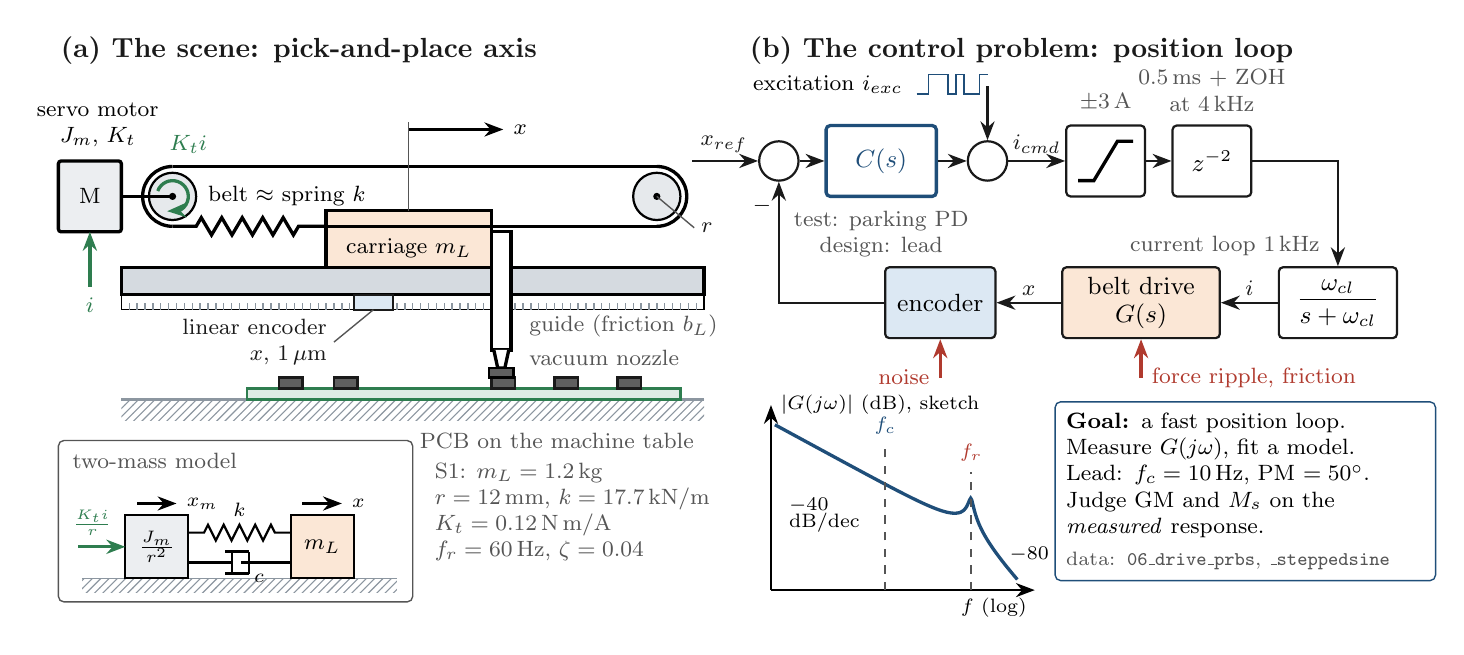
\begin{tikzpicture}
% ------------------------------------------------------------------ (a) the scene
\node[panel title] at (0,7.15) {(a) The scene: pick-and-place axis};
% PCB on the machine table
\fill[ground] (0.9,2.45) rectangle (8.3,2.72);
\draw[thick line, steel] (0.9,2.72) -- (8.3,2.72);
\draw[fill=act!15, draw=act] (2.5,2.72) rectangle (8.0,2.86);
\foreach \x in {2.9,3.6,5.6,6.4,7.2} \draw[fill=ink!70, draw=ink] (\x,2.86) rectangle ++(0.3,0.14);
\node[caption, anchor=north east] at (8.3,2.42) {PCB on the machine table};
% linear guide (rail) and encoder scale
\draw[fill=metal, thick line] (0.9,4.05) rectangle (8.3,4.4);
\draw[fill=white, thin line] (0.9,3.86) rectangle (8.3,4.05);
\foreach \x in {1.0,1.1,...,8.25} \draw[thin line, steel] (\x,3.86) -- (\x,3.95);
\node[caption, anchor=west] at (5.95,3.65) {guide (friction $b_L$)};
% pulleys and belt
\coordinate (P1) at (1.55,5.3); \coordinate (P2) at (7.7,5.3); \def\rp{0.38}
\draw[thick line] ($(P1)+(0,\rp)$) -- ($(P2)+(0,\rp)$);
\draw[thick line] ($(P1)+(0,\rp)$) arc (90:270:\rp);
\draw[thick line] ($(P2)+(0,\rp)$) arc (90:-90:\rp);
\draw[thick line] ($(P2)+(0,-\rp)$) -- (5.6,4.92);
\draw[thick line, decorate, decoration={zigzag, segment length=2.6mm, amplitude=1.1mm, pre length=3mm, post length=3mm}]
  ($(P1)+(0,-\rp)$) -- (3.5,4.92);
\foreach \P in {P1,P2} {\draw[fill=metal!60] (\P) circle (0.3); \fill (\P) circle (1.3pt);}
\node[font=\footnotesize] at (3.0,5.3) {belt $\approx$ spring $k$};
\draw[thin line, note] (P2) -- ++(-40:0.62) node[right=-1pt, font=\footnotesize, ink] {$r$};
% motor
\draw[fill=metal!45, thick line, rounded corners=1pt] (0.1,4.85) rectangle (0.9,5.75);
\draw[thick line] (0.9,5.3) -- (P1);
\node[font=\footnotesize] at (0.5,5.3) {M};
\node[font=\footnotesize, anchor=south, align=center] at (0.6,5.8) {servo motor\\$J_m$, $K_t$};
\draw[act, thick line, ->] ($(P1)+(160:0.2)$) arc (160:-110:0.2);
\node[act, font=\footnotesize, anchor=south] at ($(P1)+(0.2,0.42)$) {$K_t i$};
\draw[act, thick line, ->] (0.5,4.15) -- (0.5,4.85) node[pos=0, below, font=\footnotesize] {$i$};
% carriage clamped to the lower belt strand
\draw[fill=plantc, thick line] (3.5,4.4) rectangle (5.6,5.12);
\draw[thick line] (3.5,4.92) -- (5.6,4.92);
\node[font=\footnotesize] at (4.55,4.64) {carriage $m_L$};
% encoder read head
\draw[fill=sensorc, draw=ink] (3.85,3.86) rectangle (4.35,4.05);
\draw[thin line, note] (4.1,3.86) -- (3.6,3.45) node[left=-1pt, font=\footnotesize, ink, align=right] {linear encoder\\$x$, 1\,$\mu$m};
% pick-and-place nozzle hanging in front
\draw[fill=white, thick line] (5.6,3.35) rectangle (5.85,4.85); \draw[thick line] (5.6,4.85) -- (5.6,4.6);
\draw[fill=white, thick line] (5.63,3.35) -- (5.68,3.12) -- (5.77,3.12) -- (5.82,3.35);
\draw[fill=ink!70] (5.57,3.0) rectangle (5.88,3.12);
\node[caption, anchor=west] at (5.95,3.25) {vacuum nozzle};
% position coordinate
\draw[thin line, note] (4.55,5.12) -- (4.55,6.25);
\draw[->] (4.55,6.15) -- (5.75,6.15) node[right, font=\footnotesize] {$x$};
% two-mass inset
\begin{scope}[shift={(0.1,0.15)}]
  \draw[thin line, note, rounded corners=2pt] (0,0) rectangle (4.5,2.05);
  \node[caption, anchor=north west] at (0.05,2.02) {two-mass model};
  \fill[ground] (0.3,0.12) rectangle (4.3,0.3); \draw[thin line, steel] (0.3,0.3) -- (4.3,0.3);
  \draw[fill=metal!45] (0.85,0.3) rectangle (1.65,1.1); \node[font=\footnotesize] at (1.25,0.7) {$\frac{J_m}{r^2}$};
  \draw[fill=plantc] (2.95,0.3) rectangle (3.75,1.1); \node[font=\footnotesize] at (3.35,0.7) {$m_L$};
  \draw[decorate, decoration={zigzag, segment length=2mm, amplitude=1mm, pre length=2mm, post length=2mm}] (1.65,0.88) -- (2.95,0.88);
  \node[font=\scriptsize, above] at (2.3,0.95) {$k$};
  \draw (1.65,0.5) -- (2.2,0.5); \draw (2.2,0.38) -- (2.2,0.62); \draw (2.12,0.36) -- (2.42,0.36) (2.12,0.64) -- (2.42,0.64);
  \draw (2.42,0.36) -- (2.42,0.64); \draw (2.32,0.5) -- (2.95,0.5);
  \node[font=\scriptsize, below] at (2.55,0.48) {$c$};
  \draw[act, thick line, ->] (0.25,0.7) -- (0.85,0.7) node[pos=0.3, above, font=\scriptsize] {$\frac{K_t i}{r}$};
  \draw[->] (1.0,1.25) -- (1.5,1.25) node[right, font=\scriptsize] {$x_m$};
  \draw[->] (3.1,1.25) -- (3.6,1.25) node[right, font=\scriptsize] {$x$};
\end{scope}
\node[caption, anchor=north west] at (4.75,2.05) {S1: $m_L=1.2$\,kg\\$r=12$\,mm, $k=17.7$\,kN/m\\$K_t=0.12$\,N\,m/A\\$f_r=60$\,Hz, $\zeta=0.04$};

% ------------------------------------------------------------------ (b) the control problem
\begin{scope}[shift={(8.75,0)}]
\node[panel title] at (0,7.15) {(b) The control problem: position loop};
\def\ya{5.75} \def\yb{3.95}
\node[sum] (s1) at (0.5,\ya) {};
\node[ctrl, minimum width=14mm] (C) at (1.8,\ya) {$C(s)$};
\node[sum] (s2) at (3.15,\ya) {};
\node[block, minimum width=10mm] (sat) at (4.65,\ya) {};
\draw[thick line] ($(sat)+(-0.35,-0.25)$) -- ($(sat)+(-0.15,-0.25)$) -- ($(sat)+(0.15,0.25)$) -- ($(sat)+(0.35,0.25)$);
\node[block, minimum width=10mm] (del) at (6.0,\ya) {$z^{-2}$};
\node[block, minimum width=15mm] (cl) at (7.6,\yb) {$\dfrac{\omega_{cl}}{s+\omega_{cl}}$};
\node[plant, minimum width=20mm] (G) at (5.1,\yb) {belt drive\\[-1pt]$G(s)$};
\node[sensor, minimum width=14mm] (enc) at (2.55,\yb) {encoder};
\draw[sig] (-0.6,\ya) node[above right=-1pt, font=\footnotesize] {$x_{ref}$} -- (s1);
\draw[sig] (s1) -- (C);
\draw[sig] (C) -- (s2);
\draw[sig] (s2) -- node[above=-1pt, font=\footnotesize] {$i_{cmd}$} (sat);
\draw[sig] (sat) -- (del);
\draw[sig] (del) -| (cl);
\draw[sig] (cl) -- node[above=-1pt, font=\footnotesize] {$i$} (G);
\draw[sig] (G) -- node[above=-1pt, font=\footnotesize] {$x$} (enc);
\draw[sig] (enc) -| node[pos=0.9, left=-1pt, font=\footnotesize] {$-$} (s1);
% excitation input with a PRBS trace
\draw[sig] (3.15,\ya+0.95) -- (s2);
\begin{scope}[shift={(2.25,\ya+0.85)}]
  \draw[accent, thin line] (0,0) -- (0.15,0) -- (0.15,0.25) -- (0.4,0.25) -- (0.4,0) -- (0.5,0) -- (0.5,0.25) -- (0.6,0.25)
    -- (0.6,0) -- (0.8,0) -- (0.8,0.25) -- (0.9,0.25);
\end{scope}
\node[font=\footnotesize, anchor=east] at (2.2,\ya+0.97) {excitation $i_{exc}$};
% disturbances and noise
\draw[distsig] (5.1,\yb-0.95) node[right, font=\footnotesize, dist] {force ripple, friction} -- (G);
\draw[distsig] (2.55,\yb-0.95) node[left, font=\footnotesize, dist] {noise} -- (enc);
% annotations
\node[caption, anchor=north, align=center] at (1.8,\ya-0.5) {test: parking PD\\design: lead};
\node[caption, anchor=south, align=center] at (4.65,\ya+0.5) {$\pm3$\,A};
\node[caption, anchor=south, align=center] at (6.0,\ya+0.5) {0.5\,ms + ZOH\\at 4\,kHz};
\node[caption, anchor=south east] at (7.5,\yb+0.47) {current loop 1\,kHz};
% Bode magnitude sketch: rigid body, belt resonance, -80 dB/dec
\begin{scope}[shift={(0,0)}]
  \draw[->, thin line] (0.4,0.3) -- (3.75,0.3) node[below left=-1pt, font=\scriptsize] {$f$ (log)};
  \draw[->, thin line] (0.4,0.3) -- (0.4,2.65) node[right, font=\scriptsize] {$|G(j\omega)|$ (dB), sketch};
  \draw[accent, thick line] plot[domain=0:2.2, samples=240, variable=\u]
    ({0.45+1.4*\u}, {2.4+0.019*(-40*\u - 10*log10((1-(pow(10,\u)/60)^2)^2 + (0.08*pow(10,\u)/60)^2))});
  \draw[thin line, note, dashed] (1.85,0.3) -- (1.85,2.15) node[above, font=\scriptsize, accent] {$f_c$};
  \draw[thin line, note, dashed] (2.94,0.3) -- (2.94,1.8);
  \node[font=\scriptsize, dist, anchor=south] at (2.94,1.8) {$f_r$};
  \node[font=\scriptsize, anchor=north west, align=left] at (0.5,1.6) {$-40$\\[-2pt]dB/dec};
  \node[font=\scriptsize, anchor=west] at (3.3,0.75) {$-80$};
\end{scope}
% goal / data box
\node[draw=accent, thin line, rounded corners=2pt, fill=white, align=left, anchor=north west, font=\footnotesize,
      text width=4.55cm, inner sep=4pt] at (4.0,2.7)
  {\textbf{Goal:} a fast position loop.\\
   Measure $G(j\omega)$, fit a model.\\
   Lead: $f_c=10$\,Hz, PM $=50^\circ$.\\
   Judge GM and $M_s$ on the\\ \emph{measured} response.\\[2pt]
   {\scriptsize\color{note}data: \texttt{06\_drive\_prbs}, \texttt{\_steppedsine}}};
\end{scope}
\end{tikzpicture}
\end{document}
